\documentclass[a4paper,oneside,12pt]{report}

\usepackage{custom}

\newcommand{\barg}{\si{\bar}\text{g}} 

\usepackage{fancyhdr} 
\fancyhf{}   
\fancyfoot[C]{\thepage}                     
\renewcommand\headrulewidth{0pt}
\pagestyle{fancy}

\begin{document}

\begin{titlepage}
\hfill

\begin{center}
\Huge
\textbf{LMECA1210 - Projet en construction mécanique 1\\}
\vspace{0.5cm}
\huge
\textbf{Dimensionnement d'une bielle\\}
\Large
\vspace{0.5cm}
\textbf{année académique 2014-2015\\}
\vspace{0.5cm}
\begin{figure}[b!]
	\center
	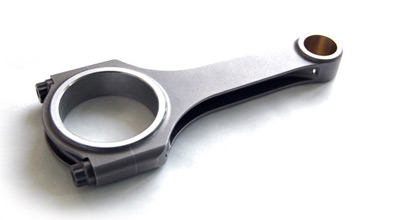
\includegraphics[width=12cm]{bielle.jpg}
\end{figure}

\end{center}
\begin{figure}[b!]
\begin{Large}
	Groupe 1\\
\end{Large}
	CHANDELLE François, 3673-13-00\\
	DISPAS David, 7189-12-00\\
	PAQUET Arnaud, 3668-13-00\\
	\\
	\newline
	\center
	
\includegraphics[width=7cm]{epl-logo.jpg}
\end{figure}
\end{titlepage}


\chapter{Réponse aux questions}

Le fonctionnement d'un moteur à explosion repose sur la conversion du mouvement alternatif du piston en rotation du vilebrequin. Cela se fait par l'intermédiaire d'une bielle. Cette pièce, répétant un cycle à raison de plusieurs milliers de fois par minute, subit des forces conséquentes. Il est donc primordial d'en faire l'analyse afin de prévoir sa forme optimale et les efforts maximaux à devoir supporter. Nous nous intéresserons ici au moteur d'une Audi A4, dont le vilebrequin nous a été confié lors des séances de mesures.

\section{Mesures}
%1. Sur base des mesures réalisées au laboratoire sur votre pièce et les pièce associée,
%déterminez les grandeurs géométriques du moteur :
%D;R;L;V
%c
%. Pour le taux de
%compression,
%$\tau$
%, une recherche personnelle est nécessaire. Il dépend de la nature
%du carburant utilisé, essence ou diesel.\\

Commençons par représenter le mécanisme qui nous intéresse: un système regroupant piston, bielle et manivelle. Cela est montré à la figure 1. \\

\begin{figure}	
	\center
	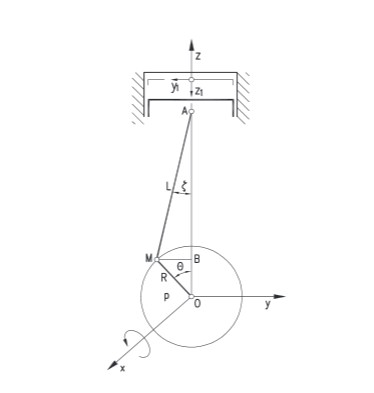
\includegraphics[scale=0.8]{Dessin.jpg}
	\caption{Piston, bielle et manivelle}
\end{figure}

Pour obtenir des résultats chiffrés, nous devons fixer les différentes longueurs. Comme dit précédemment, nous traitons ici de pièces provenant d'une Audi A4. Nous connaissons l'alésage de ses cylindres, D, et la course d'un piston, égale au double de la longueur R de la manivelle. Ces distances nous ont été fournies dans un document mis à disposition sur le site du cours. Il est possible de trouver la cylindrée unitaire $V_c$ grâce à la formule suivante: 
$$V_c =\frac{\pi D^2 R}{2}$$

En multipliant ce volume par quatre, le nombre de cylindres, nous obtenons bien la cylindrée du moteur. La longueur de la bielle, L, est quant à elle obtenue grâce à la coopération du groupe qui a hérité de la pièce durant les séances de mesures. Pour finir, ne connaissant pas précisément le modèle de la voiture, nous ne pouvons qu'estimer le taux de compression qui, rappelons nous, est le rapport du volume de la chambre de combustion lorsque le piston est au point minimum (en bas) sur le volume au point maximum (en haut). Une voiture dont le moteur fonctionne au diesel, a un taux de compression assez haut. Pour une audi A4, il avoisine 19.5 dans le cas d'une cylindrée égale à 1896 (comme pour la série 
B5\footnote{\url{http://www.auto-data.net/en/?f=showCar&car_id=4416}}). Le résumé des mesures se trouve dans le tableau 1.

\begin{figure}[h]
\centering
\begin{tabular}{|l|c|c|}
  \hline
  Longueur mesurée & Abréviation & Mesure\\
  \hline
  Diamètre du cylindre & D & $79.5mm$ \\
  Rayon de manivelle & R & $47.75mm$\\
  Longueur de la bielle & L & $199.5mm$\\
  Cylindrée unitaire & $V_c$  & $474cc$\\
  Taux de compression & $\tau$ & $19.5$\\
  \hline
\end{tabular}
\caption{Les différentes mesures}
\end{figure}

\section{Evolution de la pression}
2. Calculez l’évolution de la pression dans le cylindre en intégrant numériquement
la relation (8). Pour la phase de combustion, utilisez un angle de démarrage de
15
o
avant le PMH et une durée de
40
o
. L’énergie apportée par la combustion dé-
pend de la nature du combustible. Pour un moteur à essence prenez
2800
kJ=kg
.
Pour un moteur diesel, prenez
1650
kJ=kg
. Comme il s’agit d’un apport de cha-
leur, la masse de référence est celle de l’air dans le cylindre.
2800
kJ=kg
corres-
pond donc à
2800
kJ
par kilogramme d’air dans le cylindre. Le gaz parcourant
le cycle est supposé diatomique avec une valeur du coefficient isentropique,
,
de 1.3 pour tenir compte de l’effet de la température sur les chaleurs massiques.

\section{Efforts sur la bielle}
3. Calculez ensuite les efforts sur la bielle en fonction de l’angle de vilebrequin.
Ces efforts dépendent de la vitesse de rotation. Faites le calcul pour une vitesse
normale (3000 rpm (revolutions per minute) pour un moteur à essence et 2500
rpm pour un moteur diesel) et pour une vitesse élevée (respectivement 5000 rpm
et 4000 rpm). Illustrez l’évolution des efforts sur un cycle complet du moteur.
Cherchez les efforts maximaux et minimaux qui s’exercent sur la bielle.

\section{Justification de la forme de la bielle}
4. Justifiez la forme en "I" du corps de la bielle

\section{Dimensionnement de la bielle}
5. Dimensionnez la section de la bielle (efforts de flambage). A nouveau, une re-
cherche personnelle sera nécessaire pour faire le lien entre les forces évaluées
et la forme de la bielle. Comparez vos calculs aux mesures faites sur les pièces
réelles.

\chapter{Annexe}
Code matlab

Optionnel

\end{document}
